\documentclass{article}

\usepackage[a4paper, total={15cm, 24.5cm}]{geometry}
\usepackage{enumitem}
\usepackage{graphicx}
\usepackage[bottom]{footmisc}
\usepackage{float}
\usepackage{MnSymbol}
\usepackage{amsmath}

\title{Stochastic Model Checking of Warehouse Robotics}
\author{Corti Simone, Ravella Elia, Sarneri Enrico}
\begin{document}
	\begin{titlepage}

		\thispagestyle{empty}
		\vspace*{-1.5cm} \bfseries{
			\begin{center}
				\LARGE
				POLITECNICO DI MILANO\\
				\vspace*{.3truecm}
				
				\large				
				Department of Electronic, Information and Bioengineering\\
				\vspace*{.1truecm}
				Formal Methods for Concurrent and Real-Time Systems\\
				\vspace*{.75truecm}
				
				\begin{figure}[htbp]
					\begin{center}
						
\includegraphics[width=6cm]{./Images/logo_poli.png}
					\end{center}
				\end{figure}
				
				\vspace*{0.8cm} 
				\LARGE
				\textbf{Stochastic Model Checking of Warehouse Robotic System}\\
				\vspace*{4.5truecm}
			\end{center}
		}
		
		\mdseries
		
		\begin{center}
			\large
			Authors:\\ Corti Simone, matriculation n. 968788 \\ 
			Ravella Elia, matriculation n. 967243 \\
			Sarneri Enrico, matriculation n. \\

			\vspace*{1cm}

			Academic Year 2020-2021
		\end{center} 

    \end{titlepage}
	\clearpage
	
	\tableofcontents
	\clearpage
	
	\section{The Model}
		The final model we develepoed includes \emph{four} templates which are presented in the following section. Our design philosophy has been to make choices that are questionable from a stylistic point of view, but are ideal to overcome UPPAAL limitations and lack of optimization.
		\subsection{Grid}
			The grid is implemented as a global bidimensional array of integers. This implementation allowed us to manage in a detailed way the single cells and to simplify the movement of the bots. We did not insert a template Grid because this would have required the introduction of many additional synchronization channels and would have been very difficult to integrate with other templates.
			The integers that model the grid cells are bounded: they can only assume 8 different values. These are
			\begin{enumerate}[start=0, label={\arabic* :}]
				\item the cell is free, so no bot or pods are in that cell
				\item the cell is occupied only by a bot
				\item the cell is occupied only by a pod that is not claimed
				\item the cell is occupied only by a pod that is claimed by a task 
				\item the cell is the entry point 
				\item the cell is the delivery point
				\item the cell is occupied by a bot and a free pod
				\item the cell is occupied by a bot and a claimed pod
			\end{enumerate}
			All these slight differences among cell states are needed to safely manage the movement of the bots and the assignement of a pod to a task. Moreover, adding the last two cell states allowed us to completely remove the "Pod" template, hence making the model slimmer.\\
			The grid is highly configurable: indeed, the user is free to modify the following values:
			\begin{itemize}
				\item lenght of the grid
				\item width of the grid
				\item entry point position coloumn (can be moved along the lower edge of the grid but cannot enter the last 3 coloumns) 
				\item delivery point position coloumn (can be moved in the last three)
				\item row lenght
				\item space between rows
			\end{itemize}
			Unfortunately, Uppaal requires these parameters to be constant at compile time, so they have to be manually changed in \emph{"System declarations"}. 
			
		
		\subsection{Bot}
			The Bot template has the task to model the behaviour of the various robots in the system. \\
			It accepts as input parameter the custom-type variable $bot_t$, which represents the ID assigned to the bot.\\
			The template is composed of the following states:
			\begin{itemize}
				\item \textbf{\underline{Idle}}: this is the initial state of the template and it models the bot when it has no claimed task.\\The bot may leave this state when the number of available tasks is greater than zero. Furthermore, the probability that the bot is leaving this location is modeled as an exponential distribution with $\chi\;\sim\;(\lambda_{bot})$;
				\item \textbf{\underline{Claimed}}: this state represents the bot after it claimed a task from the queue until it reaches the delivery point. The bot is forced to leave this state after \emph{K} seconds;
				\item \textbf{\underline{Delivered}}: the bot reaches this state when its position coincides with the delivery point. The bot stays in the state until it recevies a \emph{PickUp} message from the \emph{Human};
				\item \textbf{\underline{Returning}}: after leaving the delivery point, the bot returns back to the \emph{pod position} and, after this, it goes back to the \emph{entry point}. As in claimed, the bot must leave the state after \emph{K} seconds.
			\end{itemize}
			When the pod is moving to reach its destination, it follows a predetermined path which will be explained in the following section.\\
			Notice that, inside the bot template declarations, most of the operation are carried considering booleans as integers with value of 0 or 1. This is allowed by UPPAAL and helps to reduce the effective number of states to be explored. The reason behind this is that UPPAAL \emph{if-else statements} optimization is not advanced to enough to effectively deal with all the different possible paths we needed. 
			
			\subsubsection{Movement}
				In the following, it will be presented the robot movement strategy. The main idea behind this implementation was to achieve a function pretty simple (therefore not particularly optimized), but which ensures a starvation situation is never reached.\\
				As we can see from the template, the movement of the robot is controlled by a function called \verb|chooseStrategy|. This function uses a parameter called \emph{strategy} to determine in which part of the path the robot is and to apply the corresponding movement function.
				\begin{itemize}
					\item \emph{From entry point to pod position} the bot goes to the lower left corner, reaches the row corresponding to pod one and, at the end, goes right until it reaches the pod postion.\\After reaching the pod position, the function increases by 1 the int \emph{strategy} and the boolean variable \emph{isLifting} becomes true;
					\item \emph{From pod position to delivery point} the bot follows a different strategy: after checking if the near row is free, it goes up and then left until it reaches the penultima column. Here, the bot checks wheter the cell to its left is free. If so, it goes to the left and,then, it will go up until it reaches the delivery point; otherwise it goes down and repeats this procedure at the next move.\\This system has been implemented to create an ordered queue of bot to avoid deadlocks in case of many bots inside the grid. Once it reaches the delivery point, the bot send a \emph{podDelivered} message to the human;
					\item \emph{From delivery point to pod position} the bot goes right until it reaches the ${(m-2)}^{th}$ column. Then it goes down until it reaches the line before the one it must get in. Here, the bot checks wheter the line is free. If so, it goes to the pod position following a straight path.
					\item \emph{From pod position to the entry point} the bot moves horizontally until it reaches the column corresponding to the entry point. After that, it goes down until it reaches its destination.\footnote{To avoid possible soft locking situations, in case the entry point is on the first column, the bot stops its horizontal movement at the second column, then it goes down, and eventually it moves to the right to reach the entry point.}\\This strategy features an \emph{anti-starvation} control to avoid unpredicted deadlocks.
				\end{itemize}
				The main reason behind the choice of using a single function that groups all the others was made to reduce the number of state used in the template. Note that this is a different situation with respect to \ref{sub:TaskAndHuman}.
				
				\begin{figure}[H]
					\centering
					\begin{minipage}{0.45\textwidth}
						\centering
						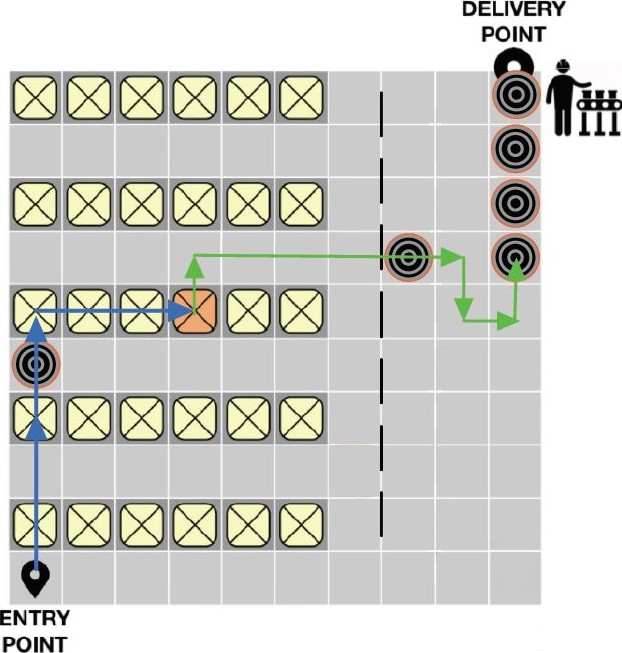
\includegraphics[width=0.9\textwidth]{./Images/BotMovement1.JPG}
						\caption{Example of bot movement between entry and delivery point.}
					\end{minipage}\hfill
					\begin{minipage}{0.45\textwidth}
						\centering
						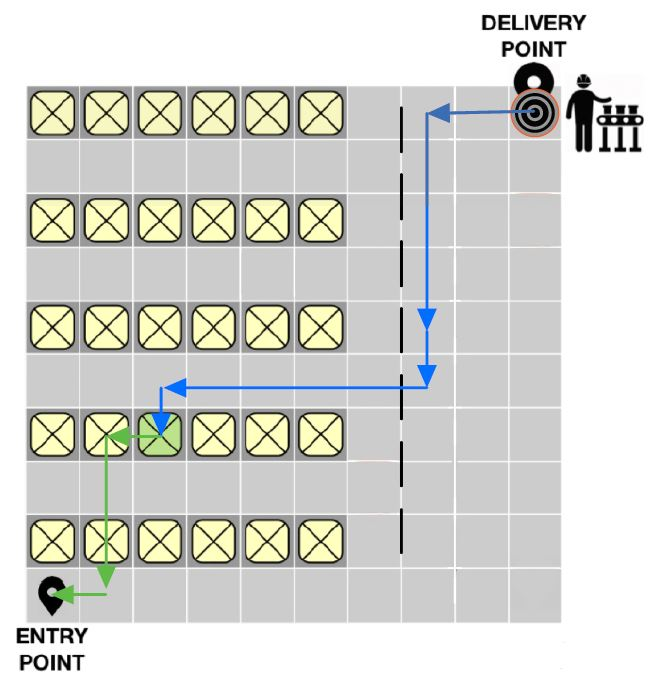
\includegraphics[width=0.9\textwidth]{./Images/BotMovement2.JPG}
						\caption{Example of bot movement between delivery and entry point.}
					\end{minipage}
				\end{figure}
				
				\begin{figure}[H]
					\centering
					\begin{minipage}{0.45\textwidth}
						\centering
						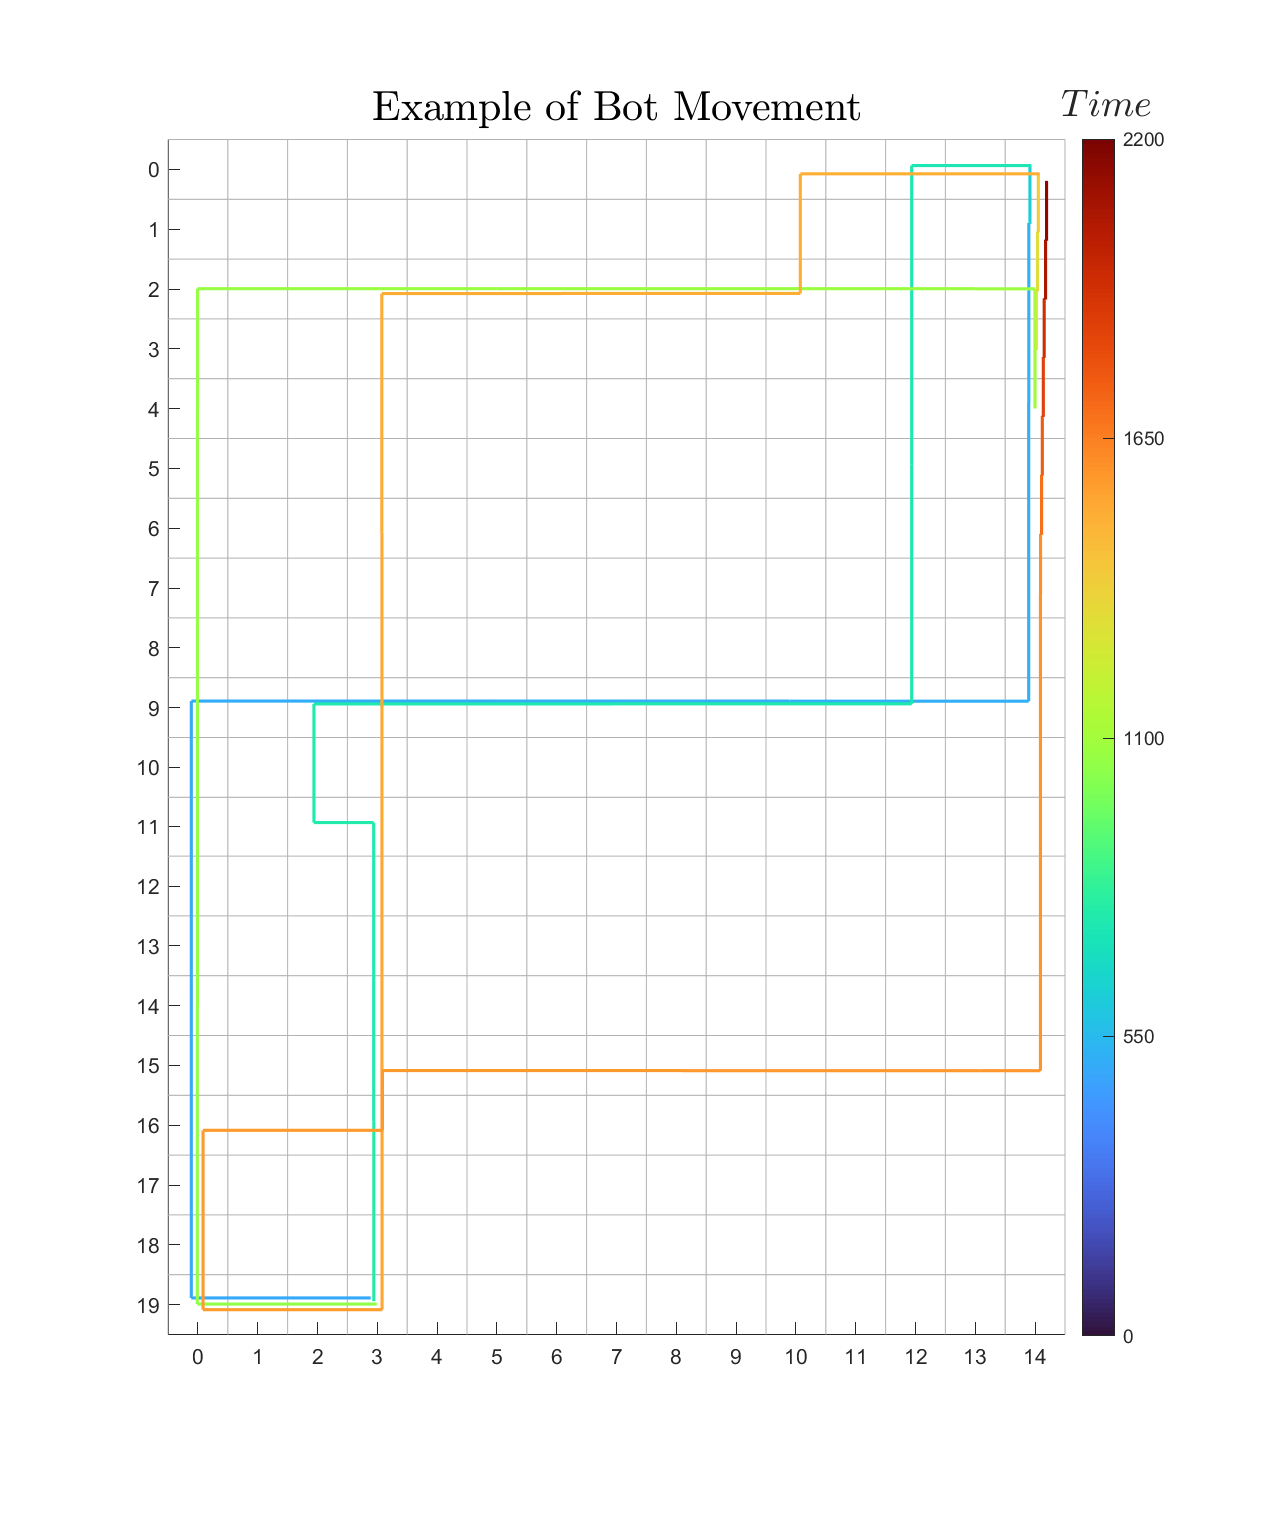
\includegraphics[width=0.9\textwidth]{./Images/BotMovement}
						\caption{Example of bot movement with $K=1\,s$ during a time of $2200\,s$.}
					\end{minipage}\hfill
					\begin{minipage}{0.45\textwidth}
						\centering
						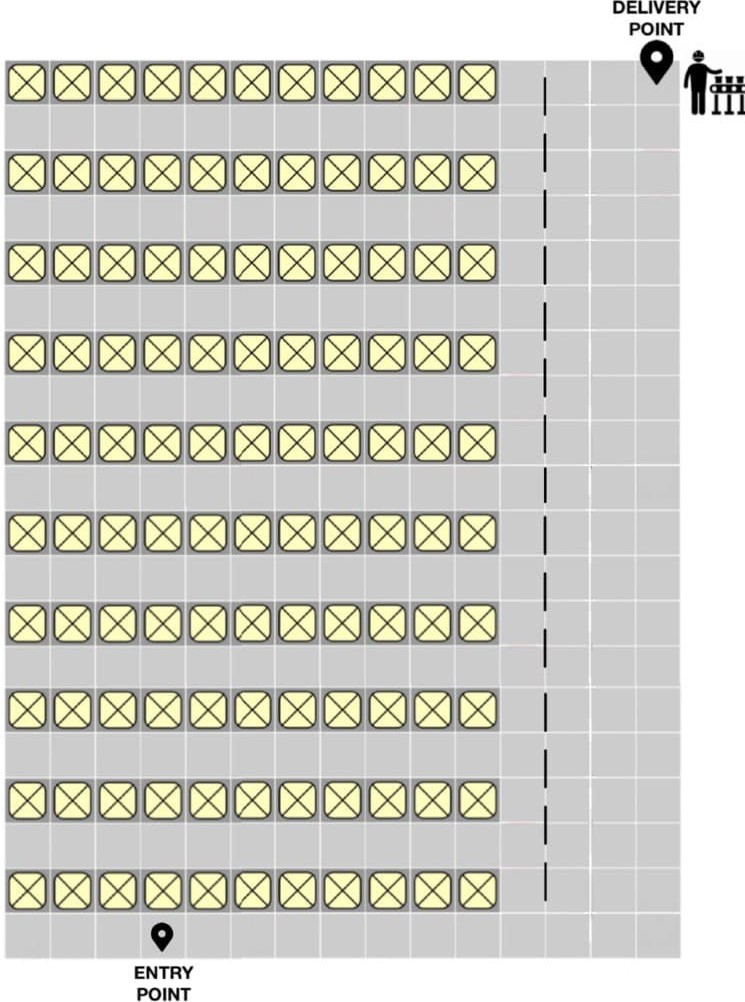
\includegraphics[width=0.9\textwidth]{./Images/Grid.jpg}
						\caption{The grid used for verification.}
					\end{minipage}
				\end{figure}

		\subsection{Queue}
			The Queue template models the mechanism to manage the arrival of new tasks in the system and their dispatching to the bots.\\
			It also carries out the grid initialization. It is composed of two states:
			\begin{itemize}
				\item An initial committed \emph{start} state that carries out the queue and grid initializations; originally, the setting of the grid was carried out by a dedicated template, but, since it was the only operation in that process, we removed it and integrated in this one in order to simplify the model. In addition, this state must be committed because no time has to pass between simulation start and various variable initialization.
				\item A \emph{working} state, whose possible transitions are used to model the following features:
					\begin{enumerate}
						\item \textbf{\underline{Adding a task to the queue}}: when the template \emph{Task} sends a token on the channel \verb|newTask|, \emph{Queue} receives it and, if the queue is not full, update the queue list; otherwise, the new task is dropped and the variable \verb|queue.discared| is increased by 1.
						\item \textbf{\underline{Communicate with BOT template}}: when a bot is sending a token on the channel \verb|claim|, \emph{Queue} receives it and communicates to the bot the task to claim, including the information about its location. In order to do so, this template updates a global variable which is accessible by the bot. In addition, when a task is claimed, \emph{Queue} updates the queue list removing the claimed task.
					\end{enumerate}
			\end{itemize}
			We have initally modelled this template with a state dedicated to each one of the function listed above, then we progressively removed the states "embedding" their functionalities in the transitions and grouping them together. 					The particular functions have been chosen because their use allowed us to reduce \emph{Queue} template to a single state, excluding the initial one. In other words, the modelled template has a very reduced number of state to be explored, increasing the overall verification performances.
		
		\subsection{Task and Human}
			\label{sub:TaskAndHuman}
			The Task template models the generation process of new tasks. Its parameters set the values of mean and standard deviation of the normal distribution associated to the "spawn rate" of new tasks.\\
			It is composed of two states:
			\begin{itemize}
				\item An initial committed \emph{startingTask} state which is in charge of initializing the additional data structures of the model, such as the list of available pods. As for the \emph{Queue} initial state, this state must be committed for the same reasons.
				\item An \emph{idle} state which just sends tokens to the channel \emph{newTask} at random time intervals, according to the distribution specified. When the timer fires, during the transition a series of updating commands are run. It is undoubt that a more elegant choice would be to use a single function where all these upgrades are grouped, however, this would have led to drop in verification performances due to UPPAAL lack of optimization.
			\end{itemize}
			The Human template, instead, models the time elapsed between the robot arrival and departure from the delivery point. Its parameters set the values of mean and standard deviation of the normal distribution associated to the time needed to complete the job.\\
			It is composed of a \emph{free} state and a \emph{busy} state to model the two possible conditions of the human operator. The transition from \emph{free} to \emph{busy} is fired when a bot reaches the delivery point and send a token on the channel \verb|podDelivered|. We decided to keep this particular channel as a single one because the human is not interested in knowing which bot delivered the pod. On the other hand, when the human completes his job, he sends a token on the channel \verb|pickUp|. Also this channel is a single one but the reason is slightly different: although it could seem useful to include the information of which bot must receive the pickUp token, it turns out this information is useless because only one bot at time may be able to receive it.\\
			The normal distribution used for the two templates has been modelled using the \emph{Box-Muller Transformation} that allowed us to transform two random uniformly distributed numbers in the interval $(0,1]$ (which are implemented in UPPAAL) into a single normal distributed numbers:
			\begin{equation}
				Z = \sqrt{-2\ln{U_1}}\,\cdot\,\cos{(2\pi U_2)}
			\end{equation}
			The choice of using the above equation has been made because of the simplicity of transforming two numbers generated using an UPPAAL built-in function into what we needed. In addition, the way to use the normal distribution probability would have been more complicated to implement and less efficient. The output of the function is a double number forced to be greater than zero. This is due to the fact that the number must be compared with a clock variable, hence it would be meaningless to use a negative value. For the comparison has been used a double number because it may be integrated in a more easy way inside the state, even if the solution is not the optimal one in terms of compatibility. Indeed, UPPAAL does not handle in a very smart way double values and raises an error when we try to use the simulator tab (no problem with the verifier instead).
			
			\begin{figure}[H]
				\centering
				\begin{minipage}{0.45\textwidth}
					\centering
					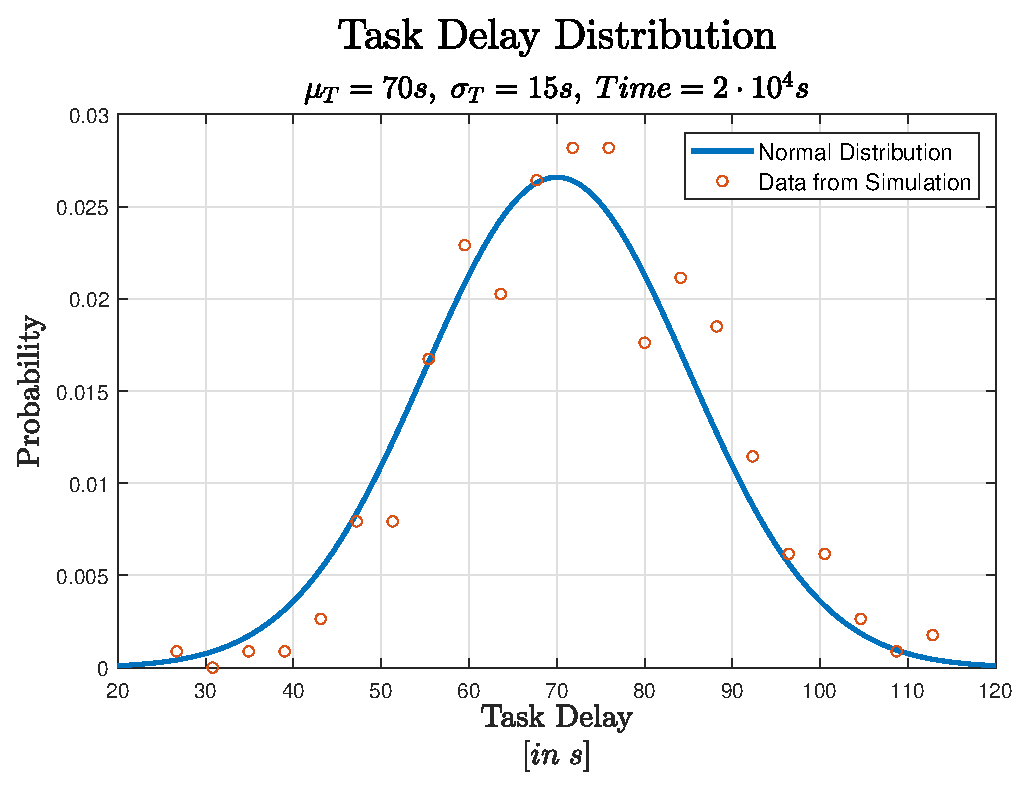
\includegraphics[width=0.9\textwidth]{./Images/taskDelay}
					\caption{Example of task delay values, compared to the theoretical distribution chosen.}
				\end{minipage}\hfill
				\begin{minipage}{0.45\textwidth}
					\centering
					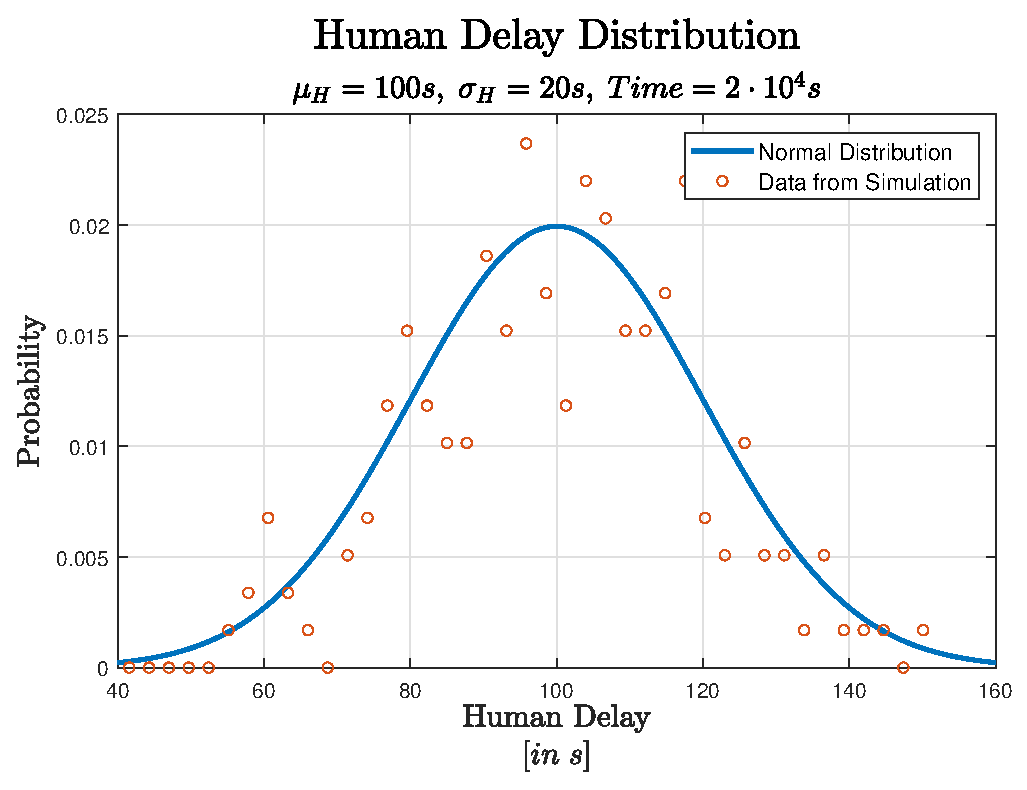
\includegraphics[width=0.9\textwidth]{./Images/humanDelay}
					\caption{Example of human delay distribution of values from the simulation.}
				\end{minipage}
			\end{figure}
			
	\section{Desired Properties}
		The crucial property the system should satisfy is that a task never get lost; this can happen only if a new task arrives and the queue is full. More formally:
		\begin{equation}
			\forall\, (\square \text{ $\neg$ (queue.discarded) } > 0)
		\end{equation}
		Since we used SMC we do not aim to get a binary "the property holds / the property does not hold" but instead a probability range that provides information about the \emph{possibility} of such condition to not hold. The parameters we have used for the statistical part of the model checking are presented in the table:
		\begin{center}
			\begin{tabular}{ | c | c |}
				\hline
				Parameter & Value \\
				\hline
				\hline
				Probabilistic deviation ($\delta$) & $\pm$ 0.01 \\
				\hline
				Probability of false negatives ($\alpha$) & 0.05 \\
				\hline
				Probability of false positives ($\beta$) & 0.05 \\
				\hline
				Uncertainty ($\epsilon$) & 0.0025 \\
				\hline
				Ratio bounds & [0.9, 1.1]\\
				\hline
				Trace resolution & 4096 \\
				\hline
			\end{tabular}
		\end{center}
		Further details in the statistical results are provided alongside the configurations.

	\section{System Configurations}
		We decided to show a schematic list of the configurations and the relative results and then put all the considerations and comments about the simulations outcome.\\
		We have prepared four configurations for the test: the first one actually fails in proving the desired property in the specified time interval, while the other ones try to fix the model changing every time a key parameter. In particular, we will try changing the human responsiveness, the number of bots and the time between two tasks.
		These parameters do not change among the various configurations:
		\begin{center}
			\begin{tabular}{ |c|c|}
				\hline
				Parameter & Value \\
				\hline
				\hline
				Grid width & 15\\
				\hline
				Grid height & 20\\
				\hline
				Number of pods per row & 11\\
				\hline
				Space between rows & 1 \\
				\hline
				Entry point position & (19, 3) \\
				\hline
				Delivery point position & (0, 14) \\
				\hline
				Maximumm queue length & 3 \\
				\hline
				Robot movement speed & 2 \\
				\hline
				Robot exponential parameter $\lambda_{bot}$ & 10 \\
				\hline
			\end{tabular}
		\end{center}
			
		\subsection{First Configuration - Failing}
			\label{sub:sim1}
			\begin{center}
				\begin{tabular}{ |c|c|}
					\hline
					Parameter & Value \\
					\hline
					\hline
					Number of bots & 8\\
					\hline
					Task spawn interval - expected value $\mu_t$ & 70\\
					\hline					
					Task spawn interval - standard deviation $\sigma_t$ & 15\\
					\hline
					Human response time - expected value $\mu_H$ & 100\\
					\hline					
					Human response time - standard deviation $\sigma_H$ & 20\\
					\hline
					Total simulation time & $5000\, s$ \\
					\hline
				\end{tabular}
			\end{center}
			\begin{figure}[H]
				\centering
				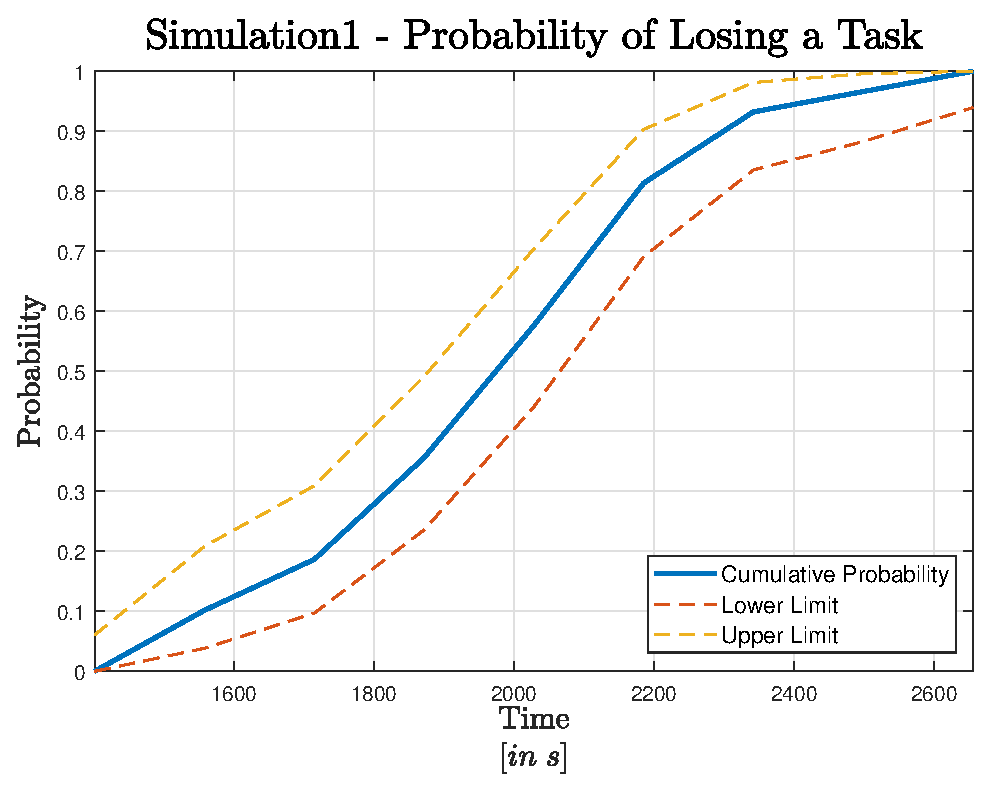
\includegraphics[scale = 0.7]{Images/Simulation1}
				\caption{Probability that a task is lost during simulation 1}
				\label{fig:sim1}
			\end{figure}
		
		\subsection{Second Configuration - Successful}
			\label{sub:sim2}
			\begin{center}
				\begin{tabular}{ |c|c|}
					\hline
					Parameter & Value\\
					\hline
					\hline
					Number of bots & 8 \\
					\hline
					Task spawn interval - expected value $\mu_t$ & 70\\
					\hline					
					Task spawn interval - standard deviation $\sigma_t$ & 15\\
					\hline
					Human response time - expected value $\mu_H$ & \textbf{60}\footnotemark\\
					\hline					
					Human response time - standard deviation $\sigma_H$ & \textbf{5}\\
					\hline
					Total simulation time & $100000\,s$ \\
					\hline
				\end{tabular}
			\end{center}
			This configuration has been verified with an upper time limit of $100000\,s$ and turned out to have a probability of losing a task lower than 5\%.
			\footnotetext{Bold numbers represent parameters changed with respect to the first configuration}	
			
		\subsection{Third Configuration - Failing}
			\label{sub:sim3}
			\begin{center}
				\begin{tabular}{ |c|c|}
					\hline
					Parameter & Value\\
					\hline
					\hline
					Number of bots & \textbf{12}\\
					\hline
					Task spawn interval - expected value $\mu_t$ & 70\\
					\hline					
					Task spawn interval - standard deviation $\sigma_t$ & 5\\
					\hline
					Human response time - expected value $\mu_H$ & 100\\
					\hline					
					Human response time - standard deviation $\sigma_H$ & 20\\
					\hline
					Total simulation time & $5000\,s$\\
					\hline
				\end{tabular}
			\end{center}
			\begin{figure}[H]
				\centering
					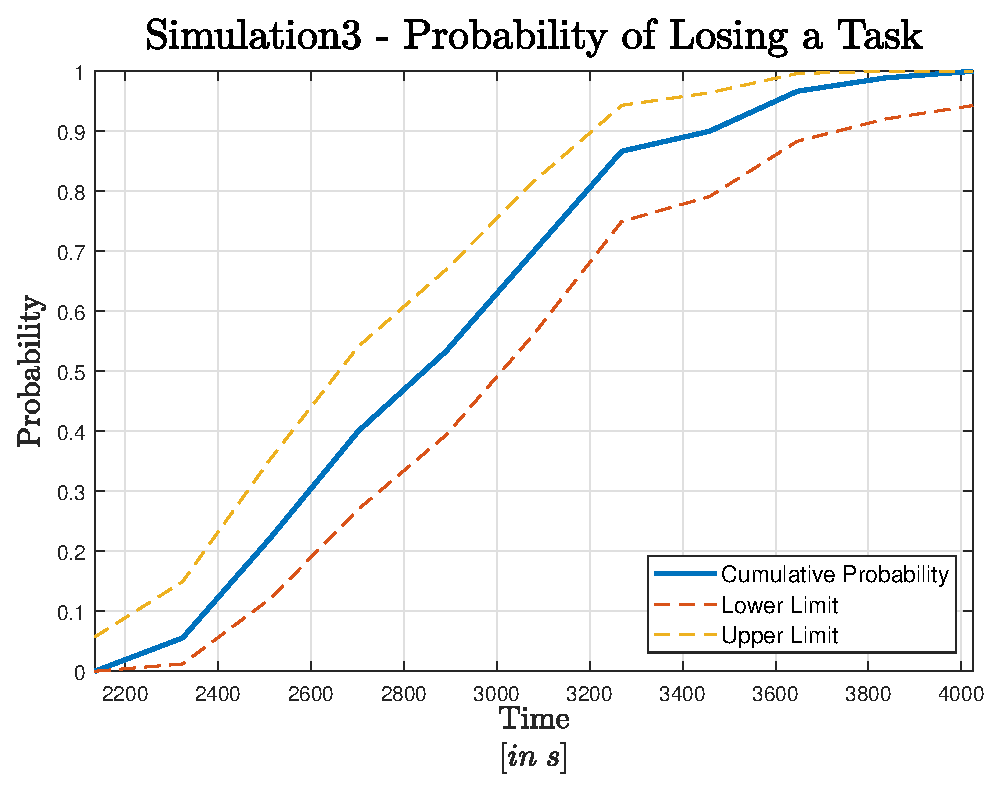
\includegraphics[scale = 0.7]{Images/Simulation3}
					\caption{Probability that a task is lost during simulation 3}
					\label{fig:sim3}
			\end{figure}


		\subsection{Fourth Configuration - Possible Failure}
			\begin{center}
				\begin{tabular}{ |c|c|}
					\hline
					Parameter & Value\\
					\hline
					\hline
					Number of bots & 8\\
					\hline
					Task spawn interval - expected value $\mu_t$ & \textbf{85}\\
					\hline					
					Task spawn interval - standard deviation $\sigma_t$ & \textbf{10}\\
					\hline
					Human response time - expected value $\mu_H$ & 100\\
					\hline					
					Human response time - standard deviation $\sigma_H$ & 20\\
					\hline
					Total simulation time & $5000\,s$\\
					\hline
				\end{tabular}
			\end{center}
			What is interesting about this configuration is that probability of failure never reach a significative value, even if it is plausible that the system would not hold. This is due to the fact that the simulation interval given is not long enough to provide significative results.
			\begin{figure}[H]
				\centering
					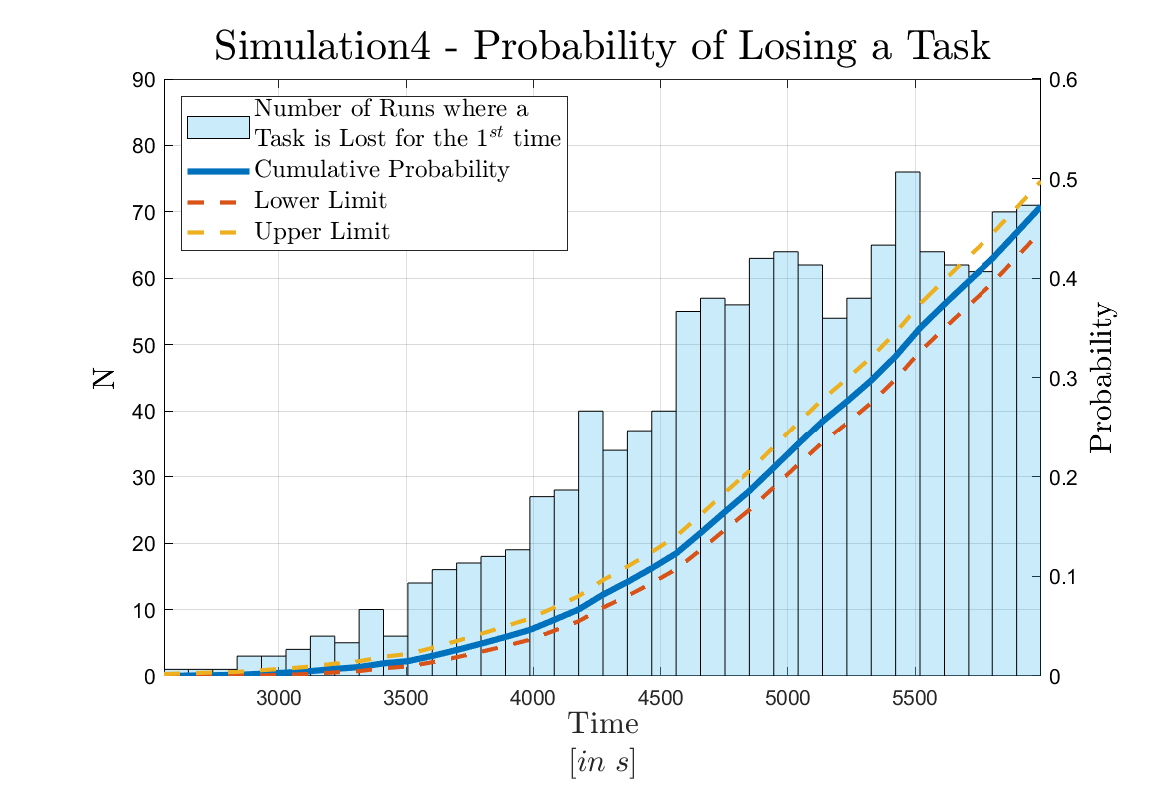
\includegraphics[scale = 0.6]{Images/Simulation4}
					\caption{Probability that a task is lost during simulation 4}
					\label{fig:sim4}
			\end{figure}
	
	\section{Result Discussion}
			As we can see from the previous section, starting from an initial configuration given by parameters such as at point \ref{sub:sim1} leads to a failure, or, in other words, to a high probability of losing a task.\\In order to avoid this, few parameter changes are made:
			\begin{itemize}
				\item {\textbf{\underline{Human Responsiveness}}: The effect of changing the time the human needs to dismiss the bot has a huge impact on the probability of success. Indeed, having a human even slightly slower than the task spawn rate leads eventually to a task lost. On the other hand, if the human is faster than the spawn rate, the success probability depends only on the time bots need to deliver a pod}
				\item {\textbf{\underline{Bot Parameters}}: Changing the number of bot inside the grid has the only effect of postponing the time of a lost task. To see this, it is sufficient to compare figure \ref{fig:sim1} and \ref{fig:sim3}. Indeed, they share a very similar probability curve, just translated along the \emph{x axis}}
				\item {\textbf{\underline{Task Spawn Rate}}:} As expected, decreasing the task spawn rate has the effect of reducing the probability of losing a task. Indeed, increasing this delay, the bots and the human have more time to complete a single task. Therefore, it is crucial not to have a spawn rate higher than the time the operator needs to complete his job
			\end{itemize}
			As we can see from the various configurations, the possible simulation outcomes are only a probability which stays below a certain value [c.f. \ref{sub:sim2}] or a probability that keeps increasing until it reaches \emph{one} [c.f. \ref{sub:sim1} \& \ref{sub:sim3}]. A probability such as the one in \emph{simulation 4} is below the unity value only because the time limit used is not high enough.
			
	\section{Conclusion}
		From the results showed, we were able to successfully find a configuration of the parameters where all the properties to check were satsified. Moreover, the configuration that we were able to test successfully used 100000 seconds to carry out the run, and that represents more than 1400\footnote{Calculated considering that, on average, a task will be added every $\mu_t$ seconds} tasks carried out.%AIUTOOOOO @Simone %PREGOOOOO @Elia 
		 Then, observing the outputs of the various configurations, we analyzed how the parameter variations affect the system itself.\\
		One of the main characteristics that emerged is the need of having the interval between tasks longer than the human response time: the operator turned out to be the main bottleneck of the system.\\
		On the other hand, we discovered that the bot number has a reduced impact on the model feasibility: having a high number of robots in the system does not modify \emph{directly} the probability of losing a packet, but extends the time needed to lose one [c.f. \ref{sub:sim1} \& \ref{sub:sim3}]. This is again due to the limits of the human operator: increasing the number of robots does not decrease the possibility of dropping a task because all of the bots will eventually have to interface with the human, and so the total service time will still heavily depend on the operator response time. A possible solution we envisioned is to add an additional operator at the same delivery point or in a different one, in order to increase system efficency.
	
	\section{Bibliography}
		\begin{itemize}
			\item \emph{A Tutorial on Uppaal 4.0} by Gerd Behrmann, Alexandre David, and Kim G. Larsen \\
				Consulted for the modeling suggestions and design patterns.
			\item \emph{Uppaal SMC Tutorial} by Alexandre David, Kim G. Larsen, Axel Legay, Marius Mikučionis, and Danny Bøgsted Poulsen \\
				Helped us with the stochastic features of Uppaal.
			\item \verb|https://docs.uppaal.org/| \\ the official software documentation for the modeling tool.
		\end{itemize}
		
\end{document}
